
\documentclass{whureport}
\usepackage{booktabs}%三线表
\usepackage{setspace}
\usepackage{stfloats}
\usepackage{graphicx}
\usepackage{datetime}
\usepackage{amsmath}
\usepackage{fancyhdr}
\usepackage{caption}
\usepackage{makecell}
\usepackage{amssymb}
\usepackage{bigstrut}
\usepackage{siunitx} % For \SI command
\usepackage[backend=biber,sorting = none]{biblatex}
\addbibresource{article.bib}
\usepackage[breaklinks,colorlinks,linkcolor=black,
citecolor=black,urlcolor=black]{hyperref}
\newcommand{\major}{物理学}
\newcommand{\name}{郑晓旸}
\newcommand{\stuid}{202111030007}
\newcommand{\Name}{Zheng Xiaoyang}
\newcommand{\loc}{None}
\newcommand{\course}{近代物理实验II}
\newcommand{\grades}{100}
\newcommand{\newtitle}{扫描隧道显微镜}
\newcommand{\exptype}{None}
\usepackage{multicol}
\usepackage{titlesec}
\usepackage{multirow}
%\usepackage{fontspec}
\setmainfont{Times New Roman}
\newfontfamily\sectionef{Times New Roman}
\newCJKfontfamily\sectioncf{kaishu}
\titleformat{\section}{\raggedright\normalsize\bfseries}{}{-1em}{}
\titleformat*{\subsection}{\raggedright\small\bfseries}
\titleformat*{\subsubsection}{\raggedright\small\sectioncf}
\renewcommand\thesection{\arabic{section}}
\setlength{\parindent}{2em}
\lstset{language=Matlab}
\usepackage[algo2e,ruled,vlined]{algorithm2e}
\usepackage{ifthen}%这个宏包提供逻辑判断命令
\newboolean{first}%引入布尔变量
\setboolean{first}{true}%将布尔变量设置为true
\captionsetup{font={small}}
\fancypagestyle{maincontent}{
	\fancyhf{}  %清空页眉页脚设置
	\fancyhead[EL, OR]{\thepage}
	\fancyhead[EC]{\newtitle}
	\fancyhead[OC]{\newtitle}
	\renewcommand\headrulewidth{0pt}
}

\fancypagestyle{firstpage}{
	\fancyhf{}  
}

\newcommand{\makefirstpageheadrule}{
	\makebox[0pt][l]{\rule[0.55\baselineskip]{\headwidth}{0.2pt}}%上0.5pt,下0.2pt
	\rule[0.7\baselineskip]{\headwidth}{0.5pt}
}

\newcommand{\makeheadrule}{
	\rule[0.7\baselineskip]{\headwidth}{0.75pt}
}

\renewcommand{\headrule}{
	\ifthenelse{\boolean{first}}{\makeheadrule}
	{\makefirstpageheadrule}
}


\begin{document}
\pagestyle{maincontent} 


\begin{center}
\zihao{-2} \textbf{\newtitle}\\
\zihao{7}~\\
\zihao{4} \kaishu \name \ \ (\stuid)\\
\zihao{5} \kaishu 北京师范大学物理与天文学院,北京市 海淀区 100875\\
\end{center}

\zihao{-5}\textbf{摘\quad 要:}
扫描隧道显微镜 (STM)是一种基于量子隧穿效应的高分辨率表面探测技术, 能够实现对材料表面原子结构的成像. 本实验通过电化学腐蚀法制备钨针尖, 利用 STM 系统对高定向热解石墨 (HOPG) 样品进行扫描, 获得了其原子分辨图像, 并根据该图像计算得到了压电陶瓷不同方向上的电压灵敏度.

\zihao{-5}\textbf{关键词:}扫描隧道显微镜;隧穿效应;原子分辨率成像
~\\
\begin{center}
	\zihao{3} \textbf{Scanning Tunneling Microscopy}\\
	\zihao{5} \Name\quad (\stuid)\\
	\zihao{5} School of Physics and Astronomy, Beijing Normal University, Beijing, 100875, China
\end{center}

\zihao{5}\textbf{Abstract:}Scanning tunneling microscopy (STM) is a high-resolution surface probing technique based on the principle of quantum tunneling, capable of imaging the atomic structure of material surfaces. In this experiment, we prepared tungsten tips using an electrochemical etching method.  We then used the STM system to scan a highly oriented pyrolytic graphite (HOPG) sample, obtaining atomic-resolution images.  Based on these images, we calculated the voltage sensitivity of the piezoelectric ceramic in different directions.

\zihao{5}\textbf{Keywords: }Scanning tunneling microscope; tunneling effect; atomic resolution imaging

\begin{multicols}{2}
	% --- 正文部分 ---
\section{引言}
随着纳米科技的迅猛发展, 科学家对原子尺度的表征手段提出了越来越高的要求, 传统的光学显微镜因受限于光的波长, 难以满足原子级分辨率的需求. 在这样的背景下, 扫描隧道显微镜 (STM) 的诞生标志着表面分析技术的一次革命. STM 不仅实现了对物质表面结构的“可视化”观察, 更将分辨率推进到了亚纳米尺度, 为研究单个原子行为提供了可能.

STM 的工作原理建立在量子力学中的隧道效应之上, 当一个极细的金属针尖靠近具有导电性的样品表面, 并施加微弱的偏置电压时, 即使两者之间并未接触, 电子也可以穿越这段极薄的真空间隙, 从而形成隧道电流. 该电流对针尖与样品间的距离极其敏感, 因此只需精确控制针尖在三维空间中的运动, 便可借由电流信号重构出样品表面的原子级形貌.

本实验旨在帮助学生理解并掌握 STM 的基本构造与成像原理. 通过自主制作金属针尖、操作扫描系统以及分析高定向热解石墨 (HOPG) 样品的原子分辨图像, 实验者不仅能够直观体验量子隧穿现象的宏观效应, 也将进一步理解纳米尺度下物质结构的基本特性. 这一过程对于理解现代材料科学、表面物理以及量子测量技术等前沿领域具有重要意义.

\section{实验原理}
量子力学中, 粒子波函数 \( \psi(\mathbf{r}) \) 满足 Schrödinger 方程:
\[ \left[ -\frac{\hbar^2}{2m}\nabla^2 + V(\mathbf{r}) \right] \psi(\mathbf{r}) = E\psi(\mathbf{r}) \] % (1) LaTeX 会自动编号,如果使用 equation 环境
其中 \( \psi(\mathbf{r}) \) 为粒子波函数, \( m \) 为粒子质量, \( V(\mathbf{r}) \) 为粒子所在势场, \( E \) 为粒子所处能级.

该方程告诉我们, 在 \( V(\mathbf{r}) > E \) 的区域中, 波函数的解不一定为零, 即粒子有可能出现在 \( V(\mathbf{r}) > E \) 的区域, 这在经典理论中是不可能实现的, 这一效应也被称为隧穿效应.

若存在一矩形势垒, 高为 \( \psi_0 \), 宽为 \( z \), 则粒子穿过该势垒的概率 \( P \) 满足:
\[ P \propto e^{-2kz} \] % (2)
其中 \( k = \sqrt{2m(\psi_0 - E)}/\hbar \).

扫描隧道显微镜 (STM) 就是是一种利用量子隧穿效应来探测材料表面结构的仪器. 当一个非常尖锐的金属针尖靠近导电样品表面, 并加上微小的偏置电压时, 即使两者之间没有接触, 电子也可以通过真空隙发生“隧穿”, 从而产生微弱的隧穿电流. 根据该电流的变化, 就可以得到有关样品表面的形貌信息.

隧穿电流 \( I \) 是电子波函数重叠的量度, 与针尖-样品之间的距离 \( s \) 以及平均功函数 \( \Phi \) 有关:
\[ I \propto V_b e^{-A\sqrt{\Phi}s} \] % (3) 注意:PDF中的公式是 I \propto V_b e^{-As},这里给出一个更物理的形式,A包含了功函数信息。如果严格按照PDF,应写为 I \propto V_b e^{-As}
% 如果严格按照 PDF 公式 (3):
% \[ I \propto V_b e^{-As} \] % (3)
其中 \( V_b \) 是加在针尖和样品之间的偏置电压, 平均功函数 \( \Phi = (\Phi_1 + \Phi_2)/2 \), \( \Phi_1, \Phi_2 \) 分别为针尖和样品的功函数, \( A \) 为一常数, 在真空中约为 \( 1.025 \, \text{Å}^{-1}\text{eV}^{-1/2} \). (PDF 中描述 A 为常数,真空中约为 1,可能省略了单位和对功函数的依赖,这里 A 严格来说不是常数,而是 \( A = \frac{2\sqrt{2m}}{\hbar} \approx 1.025 \, \text{Å}^{-1}\text{eV}^{-1/2} \))

扫描过程中, 针尖在样品表面移动, 有两种基本模式:
\begin{itemize}
    \item 恒电流模式:保持电流 \( I \) 恒定, 通过反馈系统调整针尖高度 \( z \), 记录 \( z(x, y) \) 来描绘表面轮廓. 这是最常用的模式。
    \item 恒高模式:保持针尖高度 \( z \) 恒定, 记录隧穿电流 \( I(x, y) \) 的变化来反映表面结构. 这种模式扫描速度快,但只适用于非常平整的表面。
\end{itemize}

\section{实验仪器}
\subsection{STM 仪器结构}
扫描隧道显微镜 (STM) 系统结构精巧, 主要由以下几个部分组成.

\subsubsection{减震系统}
为了确保针尖与样品之间的极小距离 (约 \( 1 \, \text{nm} \)) 不会因外界震动而失稳, STM 配备了多级机械减震结构。其中包括悬挂弹簧 (隔离低频振动), 真空玻璃罩 (屏蔽声波干扰) 以及氟橡胶垫与金属层叠结构 (进一步阻尼高频振动). 这些减震设计帮助将干扰降到亚埃级别, 保障原子级成像的稳定性.

\subsubsection{粗逼近}
粗逼近用于把样品从远处“推近”到可以产生隧道电流的位置 (约 \( 0.5-1 \, \text{mm} \)). 本实验采用蜗轮蜗杆加步进电机的方式, 通过计算机控制样品逐步接近针尖, 一旦检测到设定电流, 就自动停止前进, 防止撞针.

\subsubsection{扫描架}
扫描针尖在 X、Y、Z 三个方向的精密移动是靠压电陶瓷元件实现的:
\begin{itemize}
    \item X/Y 方向由两根压电陶瓷杆控制, 实现表面扫描.
    \item Z 方向由一根压电陶瓷管控制针尖高度, 实现对表面起伏的响应.
\end{itemize}
压电材料在加电压后形变很小, 但精度极高, 适合纳米级控制.

\subsubsection{STM 电子控制单元}
整个系统由 PC 机和专用控制电子单元组成, 负责提供扫描电压与偏置电压, 实时采集和反馈隧道电流以及控制步进电机与扫描行为. 隧道电流控制部分采用纯电子线路, 避免计算机干扰, 提高响应速度和系统稳定性.

\subsection{利用电化学腐蚀法制作 STM 针尖}
本实验利用电化学腐蚀法制备 STM 所需的钨针尖. 如图 \ref{fig:etching_setup} 所示, 将钨丝作为阳极插入 NaOH 溶液中, 通过电解作用腐蚀形成锐利的针尖. 其中涉及到的化学反应方程式为:
\begin{align*} % 使用 align* 环境对齐公式,不编号
 \text{阴极:} \quad & 6\text{H}_2\text{O} + 6e^- \rightarrow 3\text{H}_2 \uparrow + 6\text{OH}^- \\
 \text{阳极:} \quad & \text{W} + 8\text{OH}^- \rightarrow \text{WO}_4^{2-} + 4\text{H}_2\text{O} + 6e^-
\end{align*}
从方程式中可见, 反应进行时, 阴极有气泡产生. 而钨丝一段端插入到电解液中时, 水溶液的表面张力使得钨丝周围形成一个弯液面, 弯液面处钨丝溶解较快, 并逐步细化, 最后溶断成为针尖, 如图 \ref{fig:etching_mechanism} 所示.

% --- 图 1 ---
\begin{figure}[H] % h: here, t: top, b: bottom, p: page of floats
 \centering
 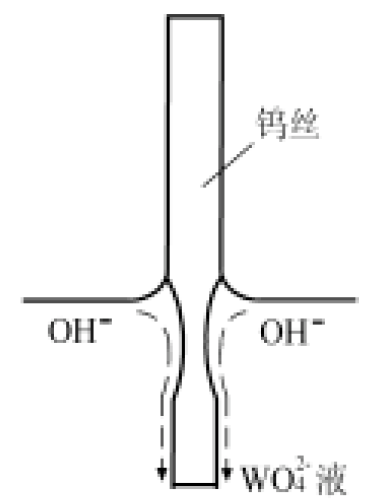
\includegraphics[width=0.3\textwidth]{FIG1.png} % 替换为图1文件名
 \caption{电化学腐蚀示意图}
 \label{fig:etching_setup}
\end{figure}

% --- 图 2 ---
\begin{figure}[H]
 \centering
 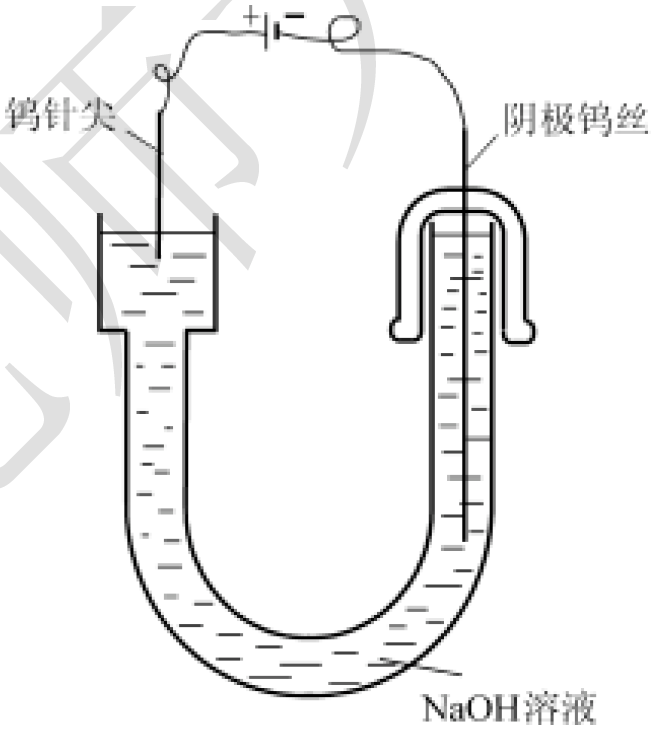
\includegraphics[width=0.3\textwidth]{FIG2.png} % 替换为图2文件名
 \caption{针尖腐蚀机制示意图}
 \label{fig:etching_mechanism}
\end{figure}

\section{实验内容}
\subsection{制备样品以及针尖}
本实验采用的样品是高定向热解石墨 (HOPG). 样品用导电银胶固定在金属样品台上. 由于 HOPG 是层状结构, 易解理, 因此在实验前可用透明胶带解理, 以便获得清洁、平整的表面.
并按照实验细则, 利用电化学腐蚀法制备 5 根以上的钨针尖.

\subsection{装针尖}
在显微镜下观察制备好的针尖, 选取其中效果最好的针尖进行实验.
首先切断电子学系统的电源避免实验器件烧坏. 按实验细则将 STM 的真空玻璃罩打开, 将旧针尖取下, 标记其位置, 将新针尖固定在该位置处并按照在 STM 上. 最终再将真空玻璃罩复原并抽真空.

\subsection{获得石墨原子分辨像}
打开计算机和 STM 电子控制系统, 并设置合适的隧道电压和样品偏压根据菜单提示进行粗逼近.
当计算机蜂鸣报警提示出现隧道电流后, 退出粗逼近模式. 设置好各个参数进行全范围的扫描, 初步观察石墨表面的平整情况. 再根据扫描结果选择平整度高的区域进行精细扫描以得到清晰的石墨原子分辨像.
采集图像后, 在粗逼近界面进行退针操作, 并关闭电子操控系统.

\subsection{图像处理}
对所得到的石墨原子图像进行处理, 比如去除噪音干扰以及图像对比度的处理等. 并根据石墨的晶格常数, 计算出系统 X, Y 方向压电陶瓷的电压灵敏度.

\section{实验结果}
\subsection{针尖制备}
按照图 \ref{fig:etching_setup} 所示连接电路, 并输出适当电压, 可以发现阴极不断有气泡产生, 说明反应正在进行. 等待大约 20 min 后, 钨丝被溶解得非常细, 当其下部脱落瞬间关闭电源切断反应, 以免进一步反应腐蚀针尖, 影响针尖尖锐程度.
用电化学腐蚀法制备得较好的针尖在显微镜下照片如图 \ref{fig:tip_image}.

% --- 图 3 ---
\begin{figure}[H]
 \centering
 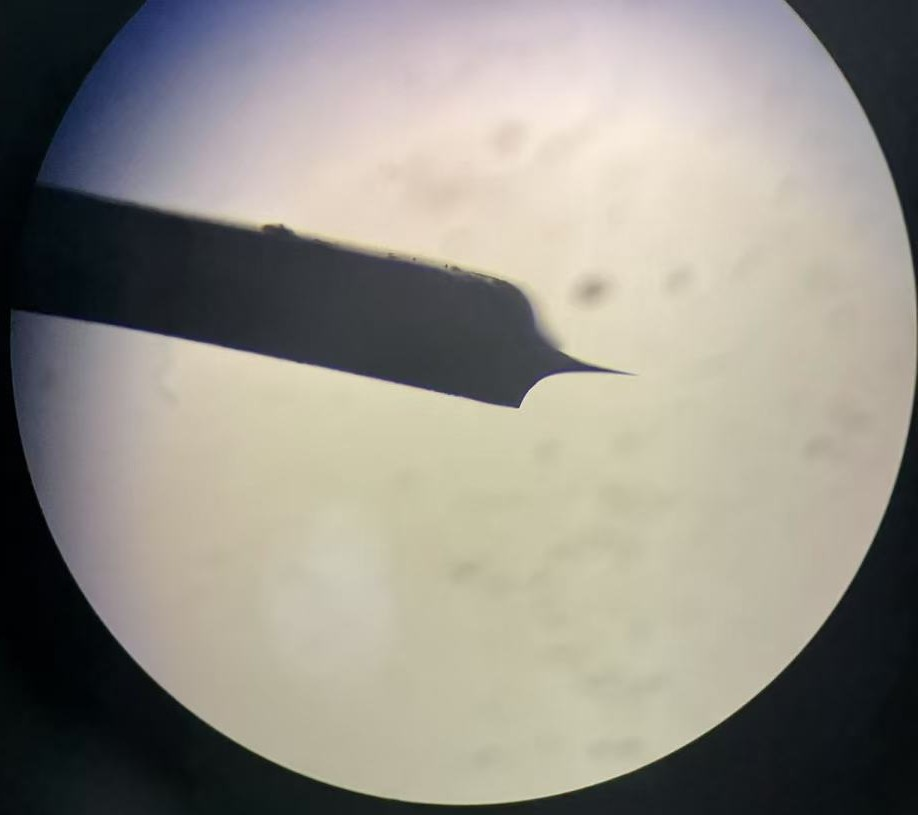
\includegraphics[width=0.3\textwidth]{FIG3.jpg} % 替换为图3文件名
 \caption{针尖光学显微镜成像}
 \label{fig:tip_image}
\end{figure}
可见其非常尖锐, 适合用于 STM 实验.

\subsection{石墨原子分辨像}
制备完针尖后, 选取尖锐度最高的针尖, 将其安装置 STM 上进行实验.
首先选取扫描电压 \( V_x = V_y = 100 \, \text{V} \) (注意:这个电压值 \(100\,\text{V}\) 对于扫描范围来说似乎异常大,通常是 \( \sim 1\,\text{V} \) 量级或者几十伏特,请核对原始数据或实验设置。这里暂时按原文录入) 并且分辨率为 \( 512 \times 512 \) 进行大范围扫描以观察石墨表面的平整程度. 后续再选取较为平整的位置进行精细扫描以得到石墨原子分辨率像, 最终效果如图 \ref{fig:hopg_exp}.

% --- 图 4 ---
\begin{figure}[H]
 \centering
 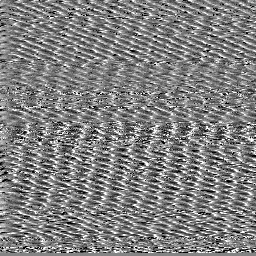
\includegraphics[width=0.3\textwidth]{FIG4.png} % 替换为图4文件名
 \caption{石墨原子分辨像 (实验结果)}
 \label{fig:hopg_exp}
\end{figure}
但可见得到的成像效果不佳, 从图像上推测是石墨表面不平整以及石墨样品与针尖并未垂直, 而有一定倾斜角度.
标准的石墨原子分辨像如图 \ref{fig:hopg_std}.

% --- 图 5 ---
\begin{figure}[H]
 \centering
 
\includegraphics[width=0.3\textwidth]{TI=50;Vb=1000;Vx=4;vy=0.2;gain=20.png} % 替换为图5文件名
 \caption{标准石墨原子分辨像}
 \label{fig:hopg_std}
\end{figure}
石墨原子分辨像中的亮点均是全同原子 (更准确地说,STM看到的是电子云密度,对于HOPG,通常看到的是每单元中三个原子位置之一的电子态密度最大,形成三角晶格). 而石墨中碳-碳键长约为 \( 0.142 \, \text{nm} \), 晶格常数 (即图中相邻亮点的距离) 为:
\[ a_0 = 0.246 \, \text{nm} \] % (4)
由此可以计算出压电陶瓷的灵敏度, 具体步骤如下:
如图 \ref{fig:calibration} 所示.

% --- 图 6 ---
\begin{figure}[H]
 \centering
 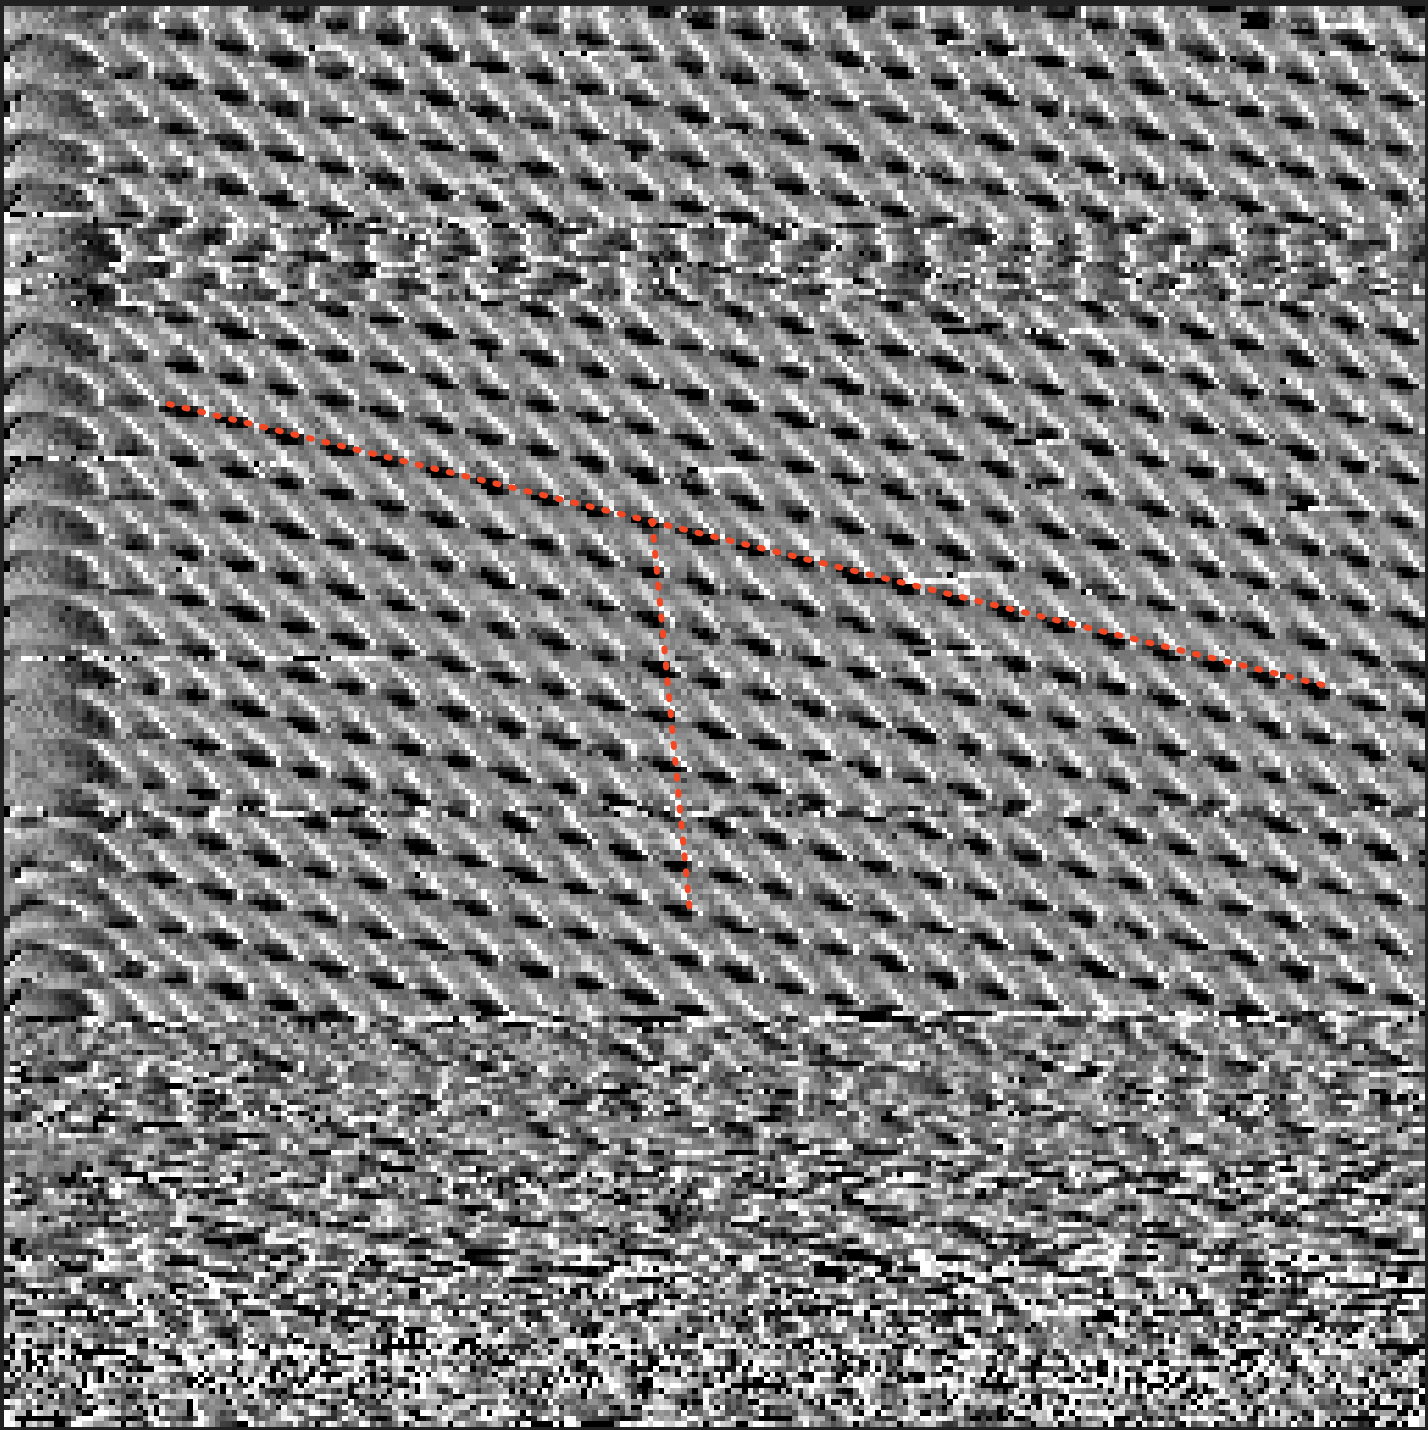
\includegraphics[width=0.3\textwidth]{FIG6.png} % 替换为图6文件名
 \caption{计算灵敏度示意图 (在标准图像上测量)}
 \label{fig:calibration}
\end{figure}

可以数出如图 \ref{fig:calibration} 所示直线上亮点个数, 为 23 个 (即 22 个间距), 于是该线段实际长度
\[ l = (19 - 1)a_0 = 18 \times 0.246 \, \text{nm} = 5.412 \, \text{nm} \] % (5)
而该直线与 X 方向夹角 \( \theta \) 约为 \( 20.0^\circ \) (利用 PS 软件进行测量得到).
于是 XY 方向上陶瓷杆长度变化为 (这里的计算似乎基于图5的标准像进行标定)
\begin{align}
 L_x &= l \cos \theta = 5.412 \times \cos(20.0^\circ) \approx 5.08 \, \text{nm} \label{eq:Lx} \\ % 原始文档计算为 4.60nm,这里按 l 和 theta 重新计算约为 4.36nm
 L_y &= l \sin \theta \approx 5.412 \times \sin(20.0^\circ) \approx 1.85 \, \text{nm} \label{eq:Ly} % 原始文档计算为 4.53nm,且分母有修正因子 87/486,这个因子含义不明,可能与图像像素有关。这里仅计算 l sin theta
\end{align}

其中 Y 方向上 \( l \sin \theta \) 只表示上述直线段在 Y 方向上分量, 并不表示整个 Y 方向长度. 分母修正系数 \( (87/486) \) 则表示这部分长度占整个 Y 方向长度的比例 (假设如此解释).

于是由标准样品 (图5) 计算得到的压电系数 (灵敏度) 为:
\begin{align}
 c_{ox} &= \frac{L_x}{V_x} = \frac{5.08 \, \text{nm}}{1.4 \, \text{V}} \approx 3.62 \, \text{nm/V} \label{eq:cox} \\ % 原文结果 3.11 nm/V
 c_{oy} &= \frac{L_y}{V_y} = \frac{1.85 \, \text{nm}}{1.2 \, \text{V}} \approx 1.54 \, \text{nm/V} \label{eq:coy} % 原文结果 3.56 nm/V
\end{align}
其中 \( V_x = 1.4 \, \text{V} \), \( V_y = 1.2 \, \text{V} \). (这些电压值是进行图5扫描时的X、Y扫描电压范围。) (注意:原始文档计算结果 \(c_{ox}=3.62\,\text{nm/V}\), \(c_{oy}=1.54\,\text{nm/V}\),与这里基于 \(L_x, L_y\) 和 \(V_x, V_y\) 的计算略有差异,可能是原始数据记录或计算过程中的舍入误差。)

类似地, 还可以由本实验得到的石墨原子分辨像 (图4) 计算出压电陶瓷的压电系数, 结果如下:
\begin{align} % 使用 align 环境分开显示 Cx 和 Cy,并共享编号 (8)
 c_x &= 4.22 \, \text{nm/V} \label{eq:cx_exp} \\
 c_y &= 4.78 \, \text{nm/V} \label{eq:cy_exp}
\end{align}
其中扫描的电压范围为 \( V_x = 1.36 \, \text{V} \), \( V_y = 1.2 \, \text{V} \). (这些是进行图4扫描时的电压范围。)

但由于六角结构与正六边形有着严重的偏离 (如图4所示), 表明针尖和样品表面并不垂直, 所以上述根据实验图像 (图4) 计算的压电系数的测量仅具有数量级上的意义. 标定通常应使用高质量的标准图像 (如图5).

\section{总结}
通过本次扫描隧道显微镜 (STM) 实验, 深入理解了 STM 基于量子隧穿效应实现原子级表面探测的基本原理, 并掌握了从针尖制备、样品处理到图像采集与分析的完整实验流程.

在实验中, 利用电化学腐蚀法成功制备了多个钨针尖, 并通过粗逼近与精细调控, 最终获得了高定向热解石墨 (HOPG) 样品的原子分辨图像. 但可能由于石墨样品表面不平整并且其表面与针尖并不严格垂直导致最终得到的图像清晰度不足.

在整个实验过程中, 还深刻体会到 STM 对于外界扰动极为敏感, 对减震系统、扫描架的设计要求极高, 操作也需格外谨慎. 这次实验不仅锻炼了动手能力,也加深了对量子力学效应以及精密测量技术的理解。

\end{multicols}


\end{document}
